%Escriba aquí su respuesta al ejercicio 6.
El algoritmo usado para la toma de tiempos es el siguiente:
\lstinputlisting[language=c]{tomaTiempos.cpp}
Para la realización de la gráfica usamos el código que hay en el \texttt{makefile} de la práctica y en el archivo \texttt{graphic.plot}:
\lstinputlisting[language=bash]{graphic.plot}
El resultado obtenido de las mediciones es el siguiente:
\begin{figure}[ht]
	\centering
	\includegraphics{graphic.eps}
\end{figure}
